\section{Résolution d'équations différentielles ordinaires}

Dans cette partie, on cherche à programmer différentes méthodes de résolution
des équations différentielles ordinaires.
Ces algorithmes utilisent tous des méthodes avec un pas de discrétisation, de la forme
$y_{n+1}=y_n+h_n \times \phi (y_n,t_n,h_n)$ .

\subsection{Représentation d'un problème de Cauchy}
Tout d'abord, on cherche à définir la façon dont on va représenter
un problème de Cauchy dans notre code. Un problème de Cauchy est défini par :
\begin{equation}
	\begin{cases}
		y(t_0)=y_0 ~\text{(condition initiale)}\\
		y’(t)=f(y(t),t) \\
	\end{cases}    
\end{equation}
Le vecteur $y_0$ représente les conditions initiales, et est modélisé en pratique par un tableau de $n$ éléments.
La fonction $y'$ donne la dérivée par rapport au temps, en fonction du temps $t$.
Pour résoudre une équation différentielle, nous chercherons donc à mettre le problème sous cette forme.

\subsection{Méthodes de résolution}
Nous avons implémenté les méthodes de résolution d’Euler, du point milieu, de Heun et de Runge-Kutta d’ordre 4.
Elles correspondent respectivement aux équations donnant $y_{n+1}$ en fonction de $y_n$, $h_n$ et $t_n$.

On a donc implémenté ces méthodes de la façon la plus générique possible. Tout d'abord, 
chaque fonction correspondant à une méthode est nommée sous la forme : \texttt{step\_method\_name(y,t,h,f)} et calcule
une unique itération de la méthode.

Nous avons ensuite implémenté \texttt{meth\_n\_step} qui calcule un nombre $N$ d'étapes avec un pas constant $h$,
puis \texttt{meth\_epsilon} qui calcule une solution approchée avec un paramètre d’erreur $\epsilon$.
En pratique, à chaque itération si l'erreur entre deux itérations successives est inférieure à $\epsilon$,
alors on arrête le calcul et on renvoie la solution.

Nous avons aussi implémenté une fonction \texttt{meth\_epsilon\_convergence} nous permettant de visualiser
sur un graphique la convergence de nos solutions.
La figure~\ref{fig:subdivision} nous montre ainsi une comparaison des résultats en fonction
du nombre de subdivisions $N$, par la méthode d'Euler.
Comme attendu, on observe une convergence de la solution vers la solution exacte (tracée en noir)
lorsque le nombre de subdivisions augmente.

\begin{figure}[htbp!]
	\centering
	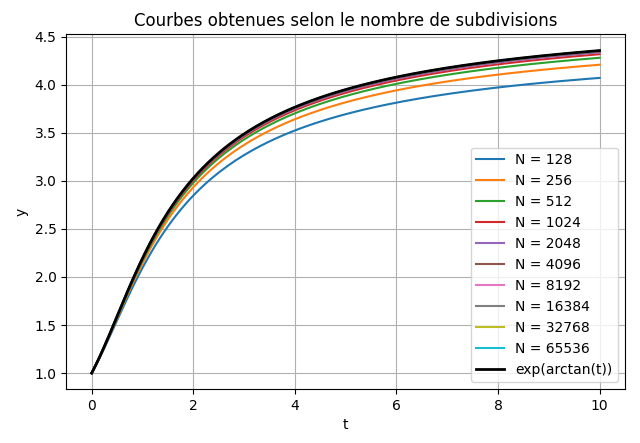
\includegraphics[width=0.5\textwidth]{res/subdivisions}
	\caption{Comparaison la convergence des solutions obtenues en fonction du nombre de subdivisions, pour l'équation différentielle $y'(t) = \frac{1}{1 + t^2}$ avec $y(0) = 1$.}
	\label{fig:subdivision}
\end{figure}

Sur l'ensemble des quatres méthodes de résolution, la plus précise est celle de Runge-Kutta, puisqu'elle est d'ordre $4$.

En revanche, elle est aussi la plus coûteuse en temps de calcul, puisqu'elle nécessite, au minimum, quatres appels à la fonction $f$ pour un unique pas de temps.

La méthode d'Euler est la moins précise (ordre $1$), mais aussi la plus rapide, puisqu'elle ne nécessite qu'un seul appel à la fonction $f$ par pas de temps.

Les autres méthodes constituent un bon compromis entre précision et temps de calcul, puisque la méthode du point milieu et celle de Heun sont d'ordre $2$, et nécessitent deux appels à la fonction $f$ par pas de temps.

\subsection{Champ des tangentes}
Pour continuer, nous avons implémenté la fonction \texttt{tangent\_2D} qui nous a permis de tracer le champ des tangentes
des équations différentielles de dimension $2$.

Comme on peut le voir sur la figure~\ref{fig:tangente}, nous avons tracé cette courbe des tangentes sur un exemple d'équation différentielle
de dimension $2$ sous la forme $y(t)=(y_1(t),y_2(t))$, avec $y(0)=(1,0)$ et $y'(t)=(-y_2(t),y_1(t))$.

Les résultats que nous obtenons pour ces champs de tangentes sont proches des résultats exacts.

\begin{figure}[htbp!]
	\centering
	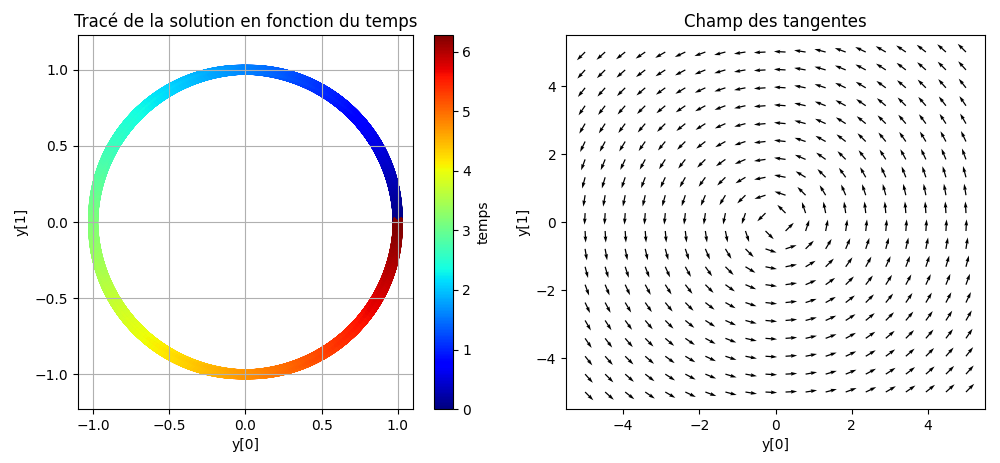
\includegraphics[width=0.7\textwidth]{res/tangente}
	\caption{Tracé de la solution de l'équation différentielle en fonction du temps, et son champ des tangentes}
	\label{fig:tangente}
\end{figure}
